\section{Results}\label{sec:results}
% Show the result/capabilities of your solution through plots, tables, screenshots, videos, etc.

Over all we are very happy with the performance of our text structure. We ran different performance metrics with a 15 KB, a 20 MB, and a 1.9 GB test file. As is visible below, we managed to implement all real time features so that all important metrics stay under 1 or 2 milliseconds, which we deem very good performance, especially since it stays in this range even with text files that are gigabytes large.
\\In figure \ref{fig:renderMetric} we show different insert patterns for the most significant cases in the 20 MB file. In this context, optimized signifies that contiguous inserts in the text sequence get merged into the same piece table piece allowing to reduce the size of the linked list in this common usage pattern (most often, text is written one char after another in our experience). We only included the metric of the 20 MB file since we didn't see a different behavior when comparing them acorss the 3 file sizes.
\begin{figure}[H]
    \centering
    \caption{gui display delay in (20 MB file)}
    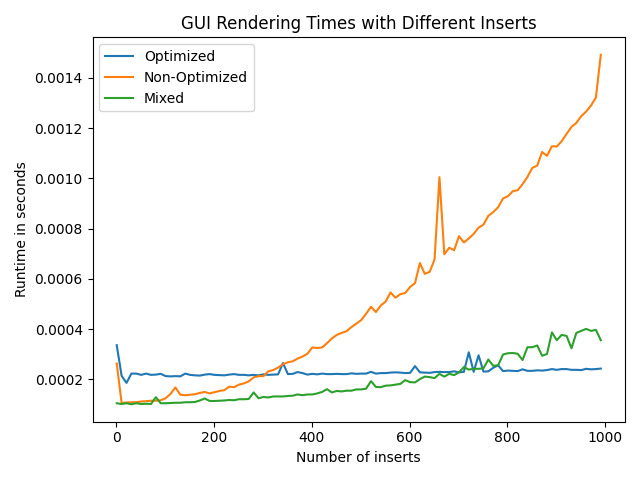
\includegraphics[width=0.6\textwidth]{./images/Profiler-Render-Metric-Size1.jpg}
    \label{fig:renderMetric}
\end{figure}
In figure \ref{fig:insertVsSize01} and \ref{fig:insertVsSize02} the average of these 3 insert patterns (at each insert position) is used to display a slowdown analysis between the three file sizes mentioned above. What is to note here, that the performance seems to be more limited by other system factors and our text structure handles inserts about as well no matter how big the file is (see average variations from one run to the other).
\begin{figure}[H]
\centering
\caption{ }
\begin{subfigure}[b]{0.48\textwidth}
    \centering
    \caption{a first metrics run}
    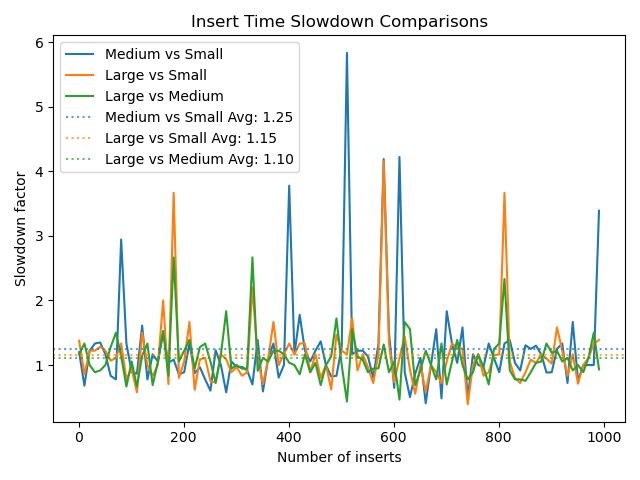
\includegraphics[width=\textwidth]{./images/Profiler-insert-slowdown-01.png}
    \label{fig:insertVsSize01}
\end{subfigure}
\hfill
\begin{subfigure}[b]{0.48\textwidth}
    \centering
    \caption{a seccond metrics run}
    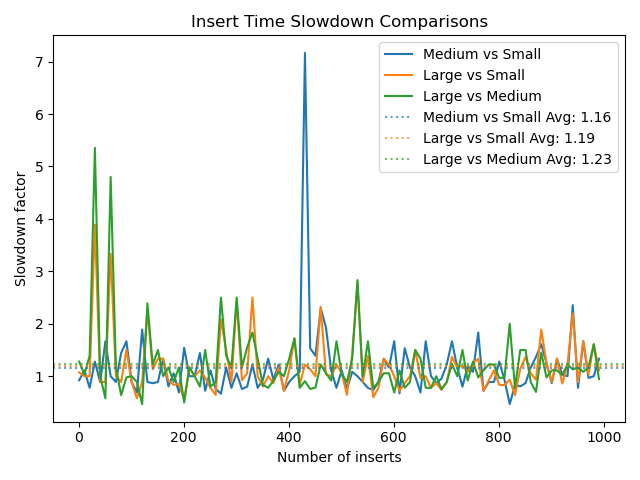
\includegraphics[width=\textwidth]{./images/Profiler-insert-slowdown-02.png}
    \label{fig:insertVsSize02}
\end{subfigure}
\end{figure}


\begin{minipage}[t]{0.48\textwidth}
\centering
\begin{figure}[H]
\centering
\caption{ }
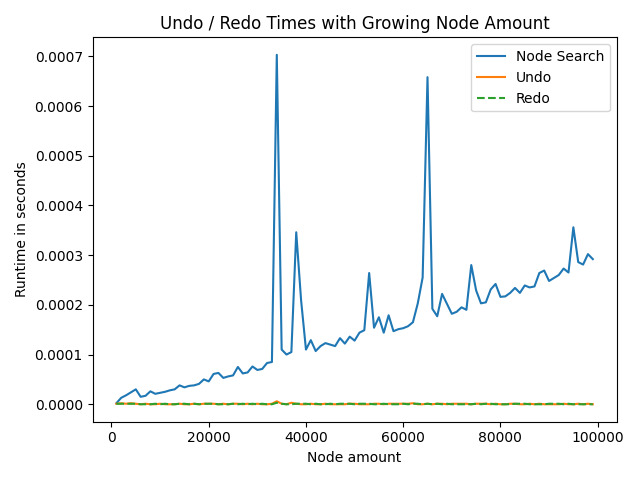
\includegraphics[width=\textwidth]{./images/Profiler-Undo-Redo.jpg}
\label{fig:undoMetric}
\end{figure}
\end{minipage}
\hfill
\begin{minipage}[t]{0.48\textwidth}
\centering
\begin{figure}[H]
\centering
\caption{ }
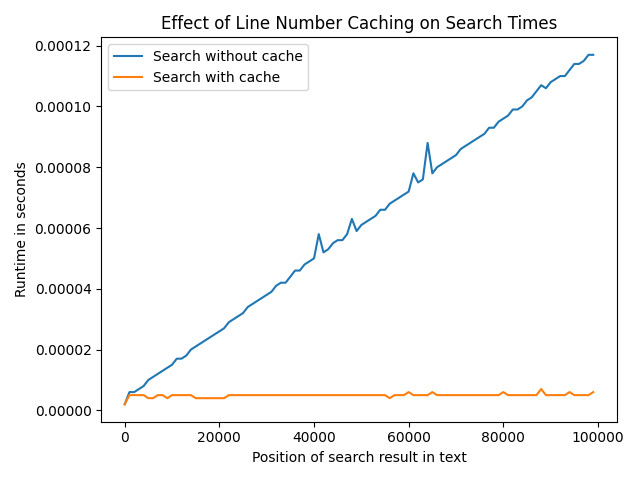
\includegraphics[width=\textwidth]{./images/Profiler-Find-Caching.jpg}
\label{fig:findMetric}
\end{figure}
\end{minipage}

%GUI
\begin{figure}[h]
    \centering
    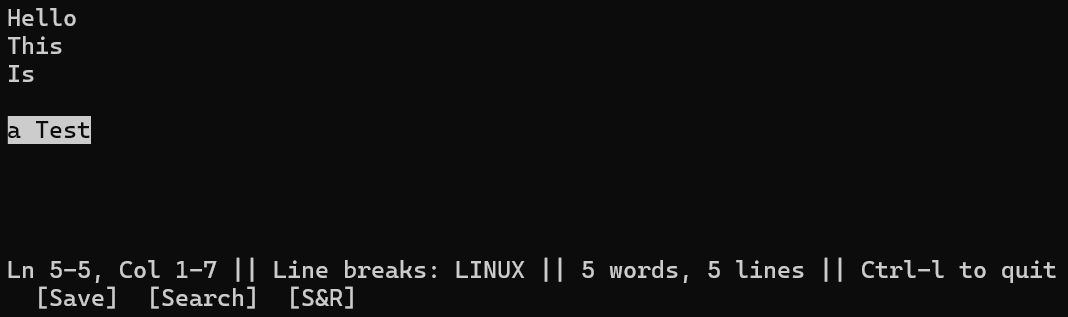
\includegraphics[width=1.0\linewidth]{figures/results_terminal.png}
    \caption{GUI of our text editor running on WSL}
    \label{fig:GUIterminal}            
\end{figure}
\noindent
Above you can see our GUI. From the top left you can see 5 lines written, one of the blank.
\\'a Test' is marked and can be use to copy/paste or delete this section.
Ln 5-5 means marked are rows from 5 to 5, same for Col but column 1 to 7.
'Line breaks: LINUX' means that the current line break style used is LINUX ($\backslash$n).
\\Next to it you also have total line and total word count and to the right is the short-cut to exit the editor.
At the very bottom are buttons that you can press to use them. S\&R means search and replace.
\\Many aspetcs of our GUI will be shown in this video \cite{demo}, as some of these things are impractical to show on a picture.